\documentclass[]{article}
\usepackage{hyperref}
\usepackage{listings}
\usepackage[bottom]{footmisc}
\usepackage{array}
\usepackage{multirow}
\usepackage[T1]{fontenc}
\usepackage{graphicx}
\graphicspath{ {./figures/} }

%opening
\title{Introduction to Computer Science and Programming in Python: VTK 2018}
\author{Ben Koger}

\begin{document}

\maketitle

\begin{abstract}
	
	\textit{ "The computer is incredibly fast, accurate, and stupid. Man is incredibly slow, inaccurate, and brilliant. The marriage of the two is a force beyond calculation." -  Einstein (maybe) }

\end{abstract}

\tableofcontents

\newpage

\section{ Introduction }

Computers are not going away.  My goal for this class is to provide a strong, general foundation upon which you can build a lifetime of programming experiences.  Understandably, many people only learn to program when there is a very specific task, like analyzing a data set, that they hope to quickly finish.  Usually, this is under time pressure, so instead of carefully taking the time to learn the best way to solve the problem, it is easier to just start googling or ask someone to show you the exact code you need to copy and paste to do exactly what you want.  The result is often that you can solve that one problem but you aren't much better off when a new, different problem comes up the next time.  I hope to take the opposite approach in this course and instead focus on slowly learning the fundamental skills that will help you solve any problem you encounter in the future quickly and efficiently. While this course will be taught using python most of the techniques will be relevant to programming in any language.       

This course if taught with the assumption of no prior programming experience.  If you have already done a some programming I hope that seeing similar ideas presented in a slightly different way will further clarify what you already know.  

The first, maybe biggest, hurdle you must get over when learning to program is convincing yourself that you can actually do it.  Unfortunately, there is a stereotype that programmers are a specific, funny group of people that like math and happen to have brains that are naturally good for programming. This, luckily, is not true.  Karlie Kloss, and Ashton Kutcher are both successful programmers. It's just one of the many things they know how to do. Once, only monks knew how to read and write and it was considered like a magical power.  Now, we all learn.  Some people learn to read faster or slower, but we all learn.   Programming is like riding a bike.  No one is born knowing how to ride a bike.  You literally have to rewire your brain to understand how balance to on two wheels. But after you practice enough and give you brain enough time adapt it feels natural. No one is born thinking like a computer. But if you practice it becomes natural. It's not embarrassing that it takes time for your brain to get used to riding a bike and it's also not embarrassing that it takes time for your brain to get used to programming.  

\section{ Hello World }

It's time to write our first program.  It won't do very much but it is always very good to start with a simple program to make sure that everything you installed for programming on your computer is working. If you have not already set up anaconda on your computer please follow the instructions at \href{https://www.anaconda.com/download/}{https://www.anaconda.com/download/} to get it working. Our first program will simply be printing out some text: "Hello World!"  In a jupyter notebook cell write the following line of code:
\begin{lstlisting}[language=Python]
    print("Hello World!")
\end{lstlisting}
When you run the cell you should see Hello World! displayed.  First program done!  Not very exciting but we're rolling. Even with just this one line program, though, we can already learn some important things about python in particular and programming languages in general. Try running that program again but with a capital P in Print.  What about getting rid of the quotation marks or parentheses?  Any on those things will break the program and you will see an error message.  First, read the error message you get in each of those cases.  You will get many more in the future so take this opportunity to see how the computer tries to tell you why the program isn't working. Second, programming languages are purposely designed to be unambiguous: for every program there can only be one way the computer will execute the code. If the computer doesn't see exactly what it expects, it will just spit out an error. It won't assume you probably meant something else, you must write in the way the computer expects.  

\section{ Variables - Numbers, Strings, and Booleans}

Variables are the simplest way that you create and store information in a program. A variable has two parts: first, the actual information that you are storing on the computer to use in your program, and second, a name that allows you to access that information whenever you want inside the program.  Variables are useful because they allow you to you the same information in multiple places in the same program.  We can incorporate variables into the Hello world program written above:
\begin{lstlisting}[language=Python]
    message = "Hello World!"
    print(message)

    > "Hello World!"
\end{lstlisting}
In the above example \textit{message} is the \textbf{name} of the variable and \textit{"Hello World!"} is the \textbf{information} that we want the computer to store to use later in the program.  You can also see that in python the equals sign (=) is used connect the name of a variable to the information you want it to refer to.  This can be confusing because it is a little different from what the equals sign means in math.  In English, you can read the line message = "Hello World!" as "message takes the value 'Hello World.'" At any one time any variable name can only be associated with one piece of information. If you use reuse a variable name the new information will replace the old information that was previously associated with the variable. For example:

\begin{lstlisting}[language=python]
    output = "Hello"
    output = "Goodbye"
    print(output)
    
    > "Goodbye"
\end{lstlisting}



There are five main types of variables in python: Numbers, strings, lists, tuples, and dictionaries.  Each of the five types of variables stores a different type of information called a \textbf{datatype}.  In this chapter we will just think about numbers and strings. We will come back to the last three in \hyperref[sec:lists-tuples-dictionaries]{another chapter}. Numbers are exactly what they sound like: 2, 89.9, and -17 are all stored as number variables in python. A string is any collection of characters that you can be typed between quotation marks on a computer.  "hi" is a string.  So are "Ls" and "I'm leaving on 12/03/2020."   

Here is a program that creates lots of variables and then prints them out.  Notice than variables can be printed out multiple times and in any order after they have been created. Variables can also be created at any point in the program - not just at the beginning.

\begin{lstlisting}[language=Python]
    a_number = 12
    test = "It's working"
    print(a_number)
    print(a_number)
    my_name = "Ben"
    print(my_name)
    print(test)
\end{lstlisting}

To most efficiently store information in a computer's memory the computer will store different types of information in different ways.  Usually you don't have to worry about how the computer stores the information you give it, but to understand how numbers work in most programming languages you do. There are four different types of numbers in python: ints, longs, floats, and complex numbers. In this course we will only use ints and floats.  All you need to know about longs and complex numbers for now is that they provide added flexibility in representing numbers in special circumstances.  \textbf{int} stands for integer and is the datatype used to store any integer (whole) number.  3, 0, 103984, -1, 409, and -194850394 are all integers.  \textbf{floats}\footnote{If you are curious about the origin of the word float and want to learn about the clever way decimals are stored a computer's in memory go to \url{https://en.wikipedia.org/wiki/Floating-point_arithmetic}} are the datatype used to store decimal numbers.  3.0, 47.3493, -3483294.234234, and 0.0 are all examples of floats.  Unlike many older programming languages, you don't need to explicitly tell python what kind of number variable want to create.  It will just guess based on what value you set the number variable you create. Later on there will be some examples where you need to consciously use one type of number over another.

\subsection{ Working with Variables }

Python allows you to do all sorts of different operations with the variables you create and they usually work as you'd expect.  Here is a small example program that shows ways you can use variables.

\begin{lstlisting}[language=Python]
    # create two ints
    num_1 = 10
    num_2 = 3
    # create a third int variable that is the value 
    # of the first two variables added together
    num_3 = num_1 + num_2
    print(num_3)
    > 13
    
    # print the result of multiplying num_1 and num_2
    print(num_1 * num_2)
    > 30
    # create a float variable
    another_number = 1.5
    # notice that we are saying that num_3 should now correspond
    # to the value of num_2 / another_number instead of the value
    # of num_1 + num_2.  We can change the value that goes with 
    # a variable name whenever we want
    num_3 = num_2 / another_number
    
    # notice also that num_3 is a float now.  
    # Any time two numbers are divided with  / symbol, 
    # the result is a float, even if the result is a whole number
    print(num_3)
    > 2.0
    
    # you can put many operations on one line
    x = 10
    y = 4.2
    z = 2
    result = x * y / (z + 5)
    print(result)
    > 6.0
    
    
    
    # now create a string type variable
    prefix_a = 'un'
    adjective = 'happy'
    
    # the only operation that can be performed on strings 
    # is called "concatenation" this is done using + symbol
    # concatenating two strings together means sicking them together
    new_word = prefix_a + adjective
    print(new_word)
    > unhappy
\end{lstlisting}

In summary:

\begin{center}
\begin{tabular}{ | m{5em} | m{5em}| m{7em} | m{20em} | } 
\hline
\textbf{variable type}& \textbf{operator} & \textbf{result} & \textbf{example} \\ 
\hline
\multicolumn{4}{|l|}{numbers} \\
\hline
 & + & addition & \begin{lstlisting}[language=python]
    x = 2
    y = 1.5
    print(x + y)
    > 3.5
\end{lstlisting} \\ 
\hline
 & - & subtraction & \begin{lstlisting}[language=python]
    x = 2
    y = 1.5
    print(x - y)
    > 0.5
\end{lstlisting} \\ 
\hline
 & * & multiplication & \begin{lstlisting}[language=python]
    x = 2
    y = 1.5
    print(x * y)
    > 3.0
\end{lstlisting} \\ 
\hline

 & / & division & \begin{lstlisting}[language=python]
    x = 2
    y = 1.5
    print(x / y)
    > 1.333333
\end{lstlisting} \\ 
\hline

 & ** & exponent & \begin{lstlisting}[language=python]
    x = 2
    y = 1.5
    print(x ** y)
    > 2.828427
\end{lstlisting} \\ 
\hline

 & \% & modulo & \begin{lstlisting}[language=python]
    x = 2
    y = 1.5
    print(x % y)
    > 0.5
\end{lstlisting} \\ 
\hline


\multicolumn{4}{|l|}{strings} \\
\hline
 & + & concatenate & \begin{lstlisting}[language=python]
    x = "Hi! Great to meet you, "
    y = "John."
    print(x + y)
    > Hi! Great to meet you, John.
\end{lstlisting} \\ 
\hline

\end{tabular}
\end{center}

\subsection{ Math }

If you would like to use more complicated math functions than those listed above you have to import a library called math. Below is an example of both importing the math library and then using some of the functions.

\begin{lstlisting}[language=python]
    import math
    
    demo_number = 100000
    # Get the base 10 log of the number in parentheses
    log_result = math.log10(demo_number)
    print(log_result)
    > 5
    
    num_a = 15
    # Get the square root of the number in parentheses
    root_a = math.sqrt(num_a)
    print(root_a)
    > 3.87283346207417
\end{lstlisting}

There are many other potential math functions you can use.  To see a full list look at \href{https://docs.python.org/3/library/math.html}{https://docs.python.org/3/library/math.html} 

You must remember to include the line that says \textit{import math} before you you try and use any of the special math functions.  This import statement tells the program that when you write math you are referring to this particular library of functions that are already saved on your computer.  Over time we will learn about other useful packages that also need to be imported. 

While at first it may seem annoying to have to import these extra functions it is actually very helpful for keeping programs both powerful and readable.  Python includes a lot of basic functionality automatically but forces you to import libraries that do specialized things. For instance, if you are interested in using videos in you program or maybe carefully dealing with GPS coordinates you must import them specially. As with math, every special library has a name that you use to tell the program you want to use those functions.  There are over a hundred thousand different special packages, each with a different name, that you can import in python. If all of those came included there wouldn't be any names left for your variables.   



\subsection{ Booleans }

Conditional statements rely on a new type of variable called a \textbf{Boolean}\footnote{Named for George Boole the 19th century inventor of Boolean algebra }.  Unlike numbers (ints and floats) and strings that can take on lots of different values, Boolean variables can only ever be one of two values: True, or False. Boolean variables can be assigned a value with the equals sign = just like number and string variables.  In the case of Boolean variables, however, you can only write True or False for the variables value. Unlike, strings, True and False are not in quotation marks. 
\begin{lstlisting}[language=python]
    # As before, first_boolean is the name of the variable being created
    # True is the value of the boolean variable
    first_boolean = True
    print(first_boolean)
    > True
    another_variable = True
    is_it_cold = False
    # As with numbers, booleans must be cast to strings before 
    # they can be concatenated to a string
    print("Is it cold today:' + str(is_it_cold))
    > "Is it cold today: False"
    
\end{lstlisting}

If you compare two variables of any data type, the result is a Boolean. You could ask is one variable is bigger than another.  The answer to this question will always be True or False so it makes sense to store the result as a Boolean.  Strings and numbers are compared slightly differently.

\subsection{Comparing numbers}

There are six main comparison operators for numbers:

\begin{center}
\begin{tabular}{ | m{5em}| m{7em} | m{20em} | } 
\hline
\textbf{operator} & \textbf{result} & \textbf{example} \\ 
\hline
< & less than & \begin{lstlisting}[language=python]
    x = 2
    y = 1.5
    print(x < y)
    > False
\end{lstlisting} \\ 
\hline
<= & less than or equal to & \begin{lstlisting}[language=python]
    x = 2
    y = 2
    print(x <= y)
    > True
\end{lstlisting} \\ 
\hline
> & greater than & \begin{lstlisting}[language=python]
    x = 2
    y = 1.5
    print(x > y)
    > True
\end{lstlisting} \\ 
\hline

 >= & greater than or equal to & \begin{lstlisting}[language=python]
    x = 2
    y = 1.5
    print(x >= y)
    > True
\end{lstlisting} \\ 
\hline

 == & equal to & \begin{lstlisting}[language=python]
    x = 2
    y = 1.5
    print(x == y)
    > False
\end{lstlisting} \\ 
\hline

 != & not equal to & \begin{lstlisting}[language=python]
    x = 2
    y = 1.5
    print(x != y)
    > True
\end{lstlisting} \\ 
\hline

\end{tabular}
\end{center}

Notice that slightly counter intuitively you check if two variables are equal by using two equals signs (==) in a row.  Remember that the single equals sign is used to set the value of a variable.  

\subsection{Comparing Strings}

There are many possible string comparisons, but right now we will look at four:

\begin{center}
\begin{tabular}{ | m{5em}| m{7em} | m{20em} | } 
\hline
\textbf{operator} & \textbf{result} & \textbf{example} \\ 
\hline
== & equals & \begin{lstlisting}[language=python]
    x = 'Libby'
    y = 'Andrew'
    z = x == y
    print(z)
    > False
    name = 'Libby'
    print(x == name)
    > True
    name = 'libby'
    # Notice the capitalization must match
    print(x == name)
    > False
\end{lstlisting} \\ 

 != & not equal & \begin{lstlisting}[language=python]
    x = 'Libby'
    y = 'Andrew'
    print(x != y)
    > True
\end{lstlisting} \\ 
\hline

\hline
in & is in & \begin{lstlisting}[language=python]
    x = 'Hi Mary'
    greeting = 'Hi'
    #is the value of the first string (greeting) contained in the value of the second string (x)
    says_hi = greeting in x
    print(says_hi)
    > True
\end{lstlisting} \\ 
\hline
not in & is not in & \begin{lstlisting}[language=python]
    x = 2
    y = 1.5
    print(x > y)
    > True
\end{lstlisting} \\ 
\hline


\end{tabular}
\end{center}

\subsection{Exercises}

\begin{enumerate}
    \item To begin, create some variables and print them out as shown above.  Create new variables using combinations of operators  and the variables you already created.  
    \item Create a program that converts a speed in meters per second to miles per hour.
\end{enumerate}

\section{ If Statements and For Loops}

In the previous chapter we made simple programs that did the same thing every time that it was run.  If we made a program that added two numbers together, then every time, no matter what, it added two numbers together.  The value of the number variables may change, but the action doesn't. The result is fairly simplistic programs.  In this chapter, we will learn how to use something called conditional statements.  As the name implies, these are programming commands that will produce different outcomes depending on what has already happened in the program. Imagine, for instance, a program that reports the weather but for both people in the united states, who expect the temperature to be reported in Fahrenheit, and people in the rest of the world, who expect the temperature to be reported in Celsius.  The program can begin by asking the user which units they prefer and return one type of information if they are Americans, and one type for everyone else.  Another useful program would take a list of temperature measurements in Kelvin and convert each to the equivalent temperature in Celsius.  Conditional statements rely on Boolean variables: when a given Boolean variable is True, do one thing, when that same variable is False, do something else instead.

\subsection{ The if statement }

The first conditional statement we will look at in detail, the if statement, is also the most straight forward.  The program will choose one of two possible actions based on the value of a Boolean.  Here is an example:

\begin{lstlisting}[language=python]

# create two number variables
price = 10.5
offer = 15.0

if offer > price:
    print('Congratulations! You can buy it.')
    
output: Congratulations! You can buy it.
    
\end{lstlisting}

In this example offer > price is the condition.  If that condition is True, then the program will do what follows in the next indented lines and then continue with the next lines in the program. If the condition is False, then the program will skip the indented lines and continue with the next unindented lines in the program. Notice also that the condition must be followed by a colon (:).

There are two other commands that are used with if statements: else, and elif. Else is used to specify what the program should do if the condition used in the if statement is False.  It looks like this:

\begin{lstlisting}[language=python]

# create two number variables
price = 10.5
offer = 5.0

if offer > price:
    print('Congratulations! You can buy it.')
    
else:
    print('Sorry, you didn't offer enough money')
    print('You need to offer ' + str(price - offer) + ' more.'

program output: Sorry, you didn't offer enough money
                You need to offer 5.5 more.
\end{lstlisting}

Notice that there is no conditonal statement after else, only after if. This is because the else statement will execute in every case that the if statement doesn't. The logic sounds like this: "If my condition is True, do this, otherwise, do this other thing instead."  As with the if statement, else statement is followed with a colon (:) and affects the following indented lines. You can only use else after an if statement. Since an else statement is defined to run when the condition of an if statement is not met, it doesn't have meaning by itself.

Elif, the last statement that can be used with if statements, is a combination of if and else.  This is used when you have three or more exclusive conditions you want the program to choose between.  Here is an example:

\begin{lstlisting}[language=python]

# create two number variables
target = 1003
guess = 500

if guess == target:
    print('You guessed the number.')
    
elif guess > target + 10:
    print('Your guess is at least 10 too high.')

elif guess < target - 10:
    print('Your guess is at least 10 too low.')
    
else:
    print('Your guess is within 10 of the correct answer.')

program output: You guessed too low.
\end{lstlisting}

In the same way that the lines of code in the indent following the else statement run whenever the condition in the preceding if statement is not met, the indented lines of code following the elif statement run when \textit{both} all of the conditions above the current elif statement are False (the last if statement plus and following elif statements) and the condition of the current elif statement is True. The else statement conditions to run only when none of the conditions in the preceeding if and elif statements are not met. 

\subsection { While Loops }

Imagine you were a rocket scientist so you wanted a to print out a chart showing the square root of every number from 0 to 100.  You could do this alread with what you know, but it would take you 100 lines where each line you print out another value. That's very impractical.  When you go to the moon you might want a chart that goes to a million! A much better way is to use something called a while loop.  This will accomplish the same thing in just three lines of code regardless of how many square roots you'd like to print out. 

While loops let you repeat a certain block of code over and over again until you want to stop. While they seem very new, While loops are actually just like if statements but when the condition is True, after executing the indented lines, instead on continuing on with the rest of the program like with an if statement, the while loop will go back to the initial condition and if the condition is still True, repeat the process again.  For a visual representation, look at Figure ~\ref{fig:ifWhileDiagram}: 
\begin{figure}[!htb]
    \centering
    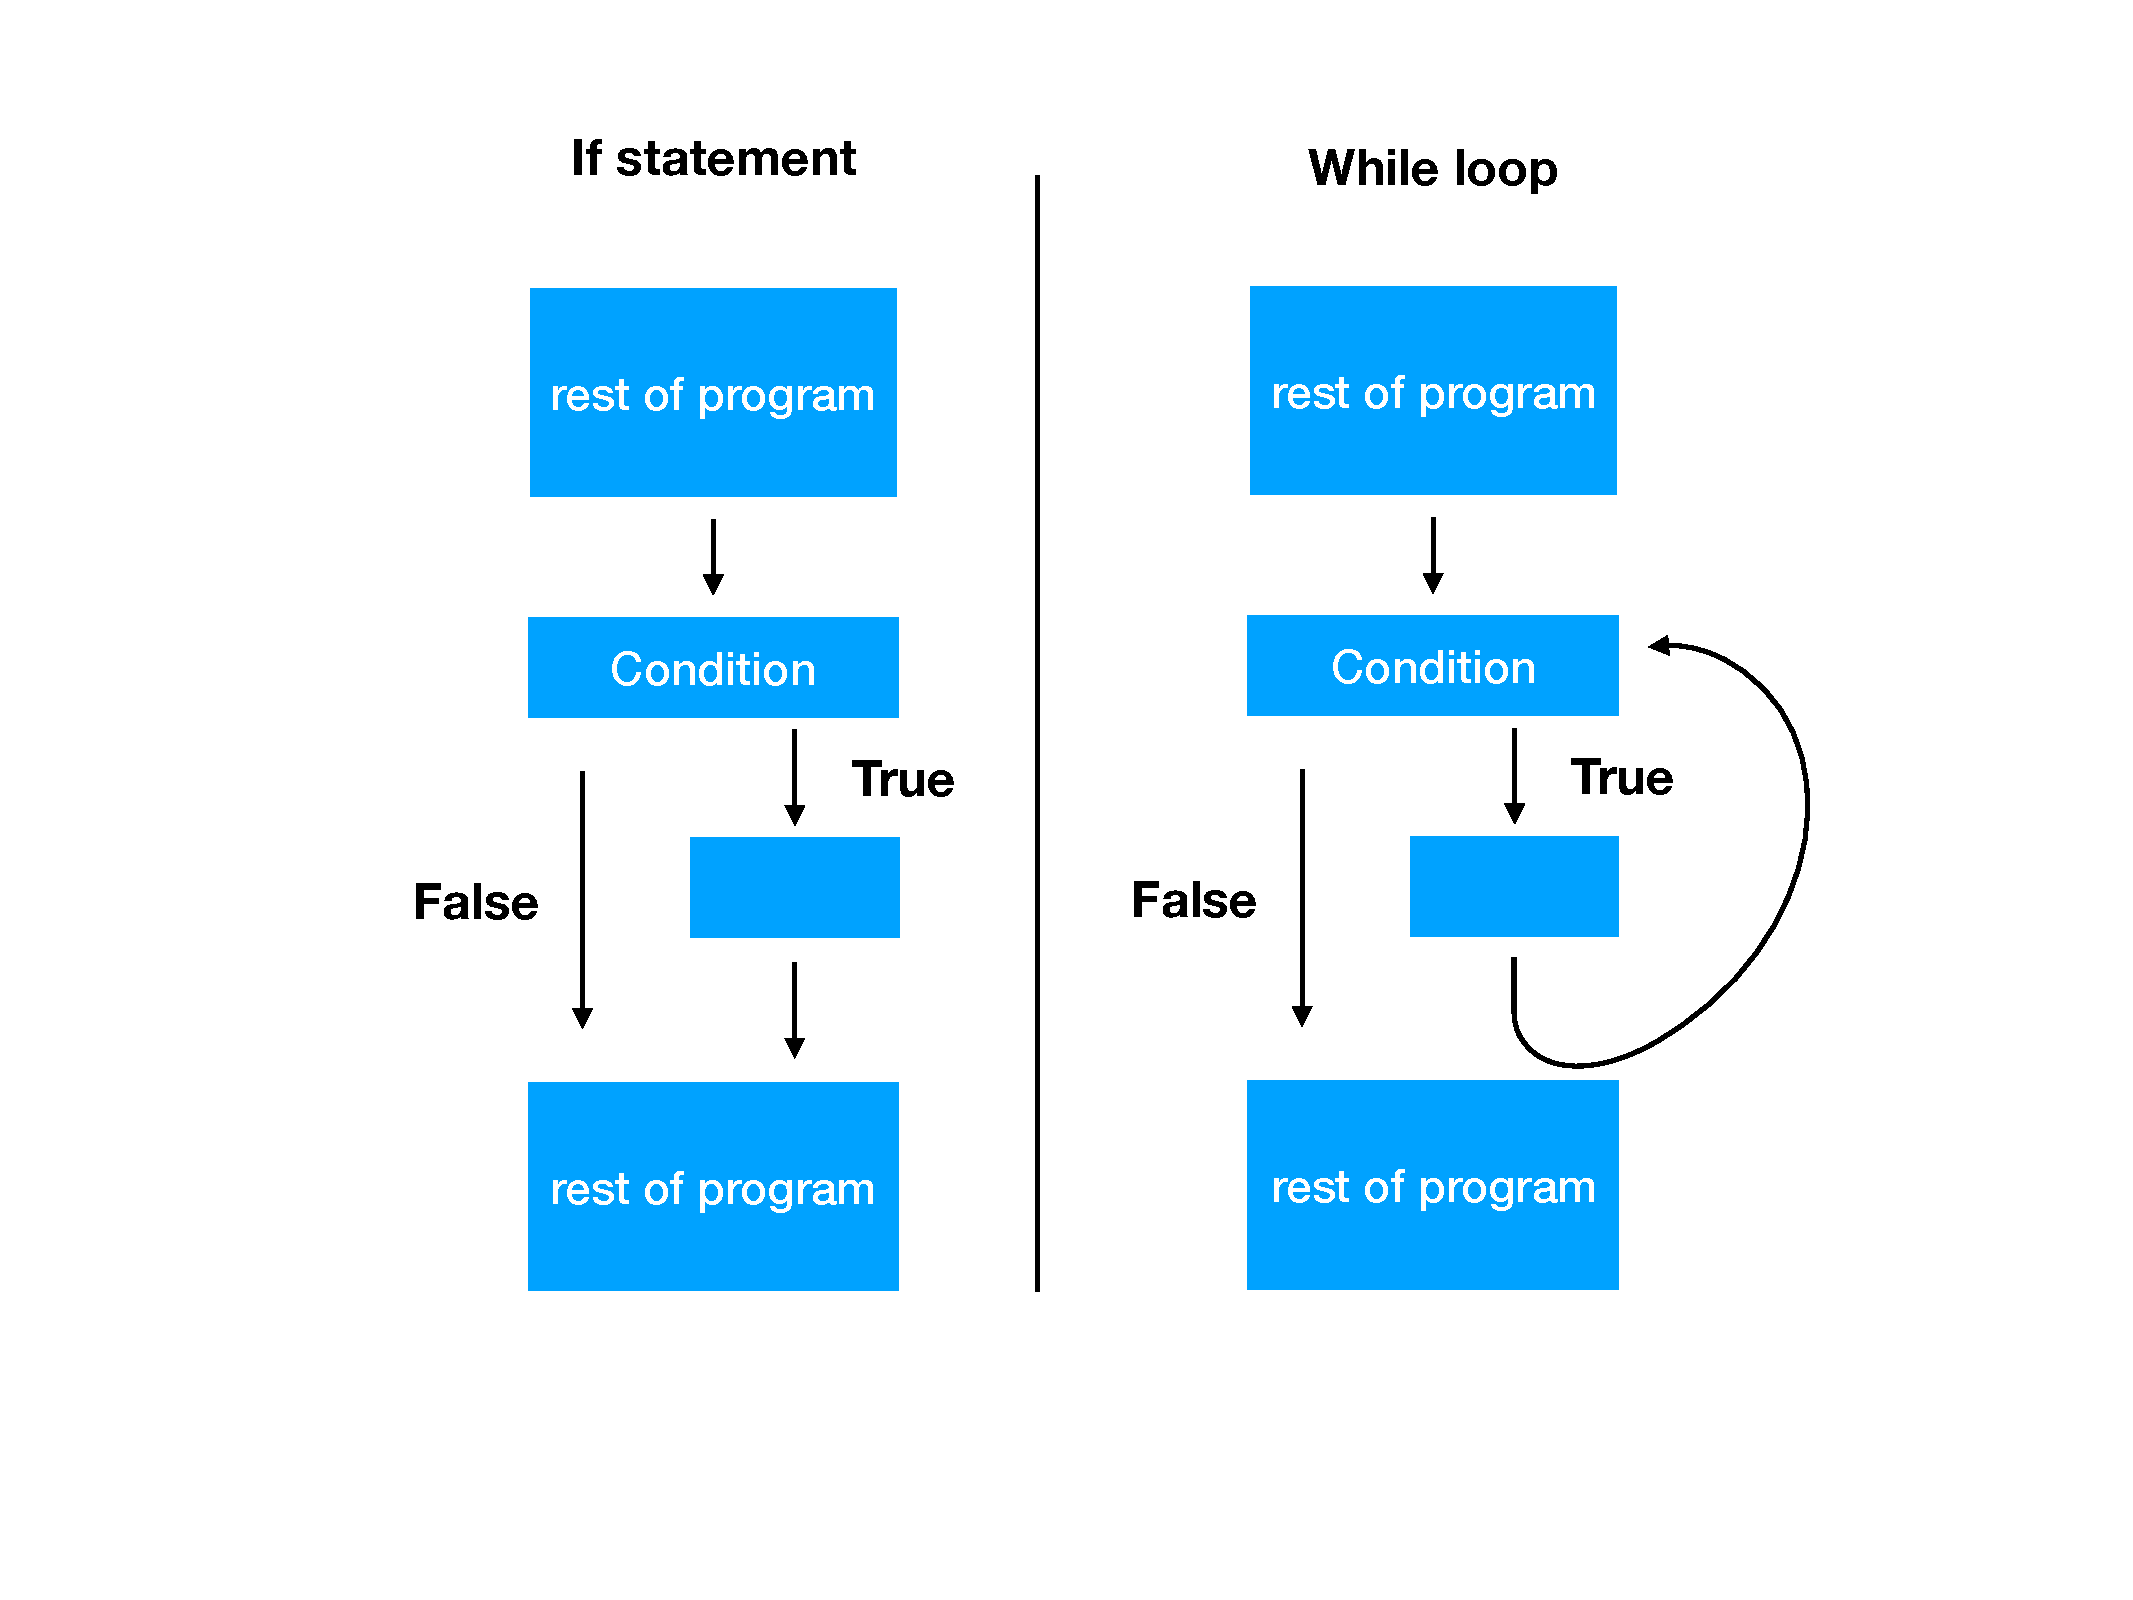
\includegraphics[width=\textwidth]{if-statement-while-loop-diagram.pdf}
    \caption{Caption}
    \label{fig:ifWhileDiagram}
\end{figure}

As you might imagine, this means the variable used in the condition of the while loop must somehow be changed by the code in the indented part of the while loop.  If not, then if the condition is True the first time then it will continue to be True every time the program loops back to the condition after finishing what's inside the loop. This can easily happen (and will surely at one point happen to you) and is called an infinite loop.  You must manually shut down the program when this happens.  Otherwise it will never finish.  Here is an example of a simple while loop that prints out the cube of every whole number from 0 to 10:

\begin{lstlisting}[language=python]
# A program the prints out the cube of
# every whole number from 0 to (but not including) 10
current_num = 0
num_cubes_to_print = 10
while current_num < num_cubes_to_print:
    cube = current_num ** 3
    print('The cube of', current_num, 'is', cube)
    current_num = current_num + 1

\end{lstlisting}

Notice how every time the program goes through the loop current\_num is increased by one.  Since the variable's value starts at 0 the while loops condition will be true for the first ten times through the loop (the value of current\_num is 0, then 1, then 2, ... then 9, all less then the value of num\_cubes\_to\_print). After the tenth run, however, current num will be 10, so the condition will no longer be true and the program will end.

While loops are particularly useful when you want the program to reach a particular result but you don't necessarily know how long it will take.  Imagine, for instance, if you wanted to simulate gambling strategies. To compare which strategy is better or worse you would want to see how long it takes to either reach some target amount of money, or loose everything.

This is easy to with for loops.

\begin{lstlisting}[language=python]

# First you need to set the parameters of the gambling game
# In this game, when you win you gain a dollar
# when you loose you loose a dollar

# The probability of winning is determined by 
# the variable named prob_win
prob_win = .3

# The starting amount of money is set by the variable
# called start_money
start_money = 500

# You also need a way to keep track of the 
# Current amount of money the user has throughout the simulation
# We'll call this curr_money and initially is should 
# be the same value as the starting money
curr_money = start_money

# The amount of money the player wants to get before stopping
goal = 1000

# The simulation should run until either the player reached 
# their goal or runs out of money
# These, therefore should be the conditions for the while loop
while curr_money != 0 and curr_money < goal:
    # first get a random float from 0 to 1
    random_draw = random.random()
    
    # based on the probability of winning specified above
    # see if the random draw resulted in a win or loss for the player
    if random_draw < prob_win:
        curr_money = curr_money + 1
    else:
        curr_money = curr_money - 1
        
# After the while loop finishes, tell the player if they won or lost
if curr_money == 0:
    print('Sorry, you lost all of your money')
else:
    print('Congratulations! You won ' + str(curr_money - start_money) + 'dollars.')
    

\end{lstlisting}

This works for simulating a single round of gambling. To test potential strategies, though, you'll want to simulate many different rounds and see what works best on average. Suppose you want to simulate 100 rounds of gambling. It would be possible to do this with another while loop.  There is slightly simpler way, however, called a \textbf{for loop}.

\subsection{For loops}

For loops are for when you want do something a known number of times. If you want to run a simulation 10 times, for example, you would use a for loop.  Maybe you want to print out the first 20 numbers in the Fibonacci sequence. If you want to run some piece of code until some event, like you run out of money in a simulation, happens, however, while loops work better. While loops and for loops are similar, but they each work more naturally in different situations. 

With while loops, you define variable, often called a counter,  before the while loop and then use that variable in a conditional statement which defines whether or not the while loop should run.  Then, within the loop, you change that variable in some why so that the loop eventually ends when the variable has been changed in a certain way.  With a for loop, however, the variable that changes during the loop is defined on the same line as the for loop. Furthermore, you don't have to explicitly change the variable every time you move through the loop. The program changes it for you. It's easiest to look at in an example.

Here's an example of doing the same thing first with a while loop and then again with a for loop:

\begin{lstlisting}[language=python]
# count out ten bananas
number_to_count = 10
#current number of bananas counted
banana_count = 0
while banana_count < number_to_count:
    print(banana_count, 'banana')
    banana_count = banana_count + 1

# Now doing the same thing but with a for loop
number_to_count = 10
for banana_count in range(number_to_count):
    print(banana_count, 'banana')
\end{lstlisting}

So changing to a for loop saves two lines of code.  More importantly, though, it combines all of the information controlling the loop in one place so it is easier to read and understand what if happening.  It will also come in handy in the next chapter when we start using lists.



Let's finish the gambling simulator from before so that we can find the average number of games it takes for us to get the money we want or loose it all. We can also get the average amount of money we have at the end of each round.

\begin{lstlisting}[language=python]
# First, define some parameters of the simulation
# The parameters defined here, outside the for loop, will
# apply to every simulation

# Number of rounds to play/simulate
num_rounds = 100

# The amount of money the player wants to get before stopping
goal = 1000

# The probability of winning individual game
prob_win = .3

# The starting amount of money
start_money = 500

# We will create two variables to store the results from all of the rounds played
# We'll use this to keep track of all the games played in all the rounds
# We begin having played 0 games 
total_games_played = 0

# We'll use this to keep track of all the money won in all rounds
# We begin having won 0 dollars
total_money = 0

# We'll use this to keep track of the number of games won
total_wins = 0

# create a for loop that will play num_rounds rounds of the gambling game
for game_num in range(num_rounds):
    # This part simulates one round of gambling as shown above
    
    # For each simulated round, the player starts with the same
    # amount of money
    curr_money = start_money
    
    # Use this variable to keep track of the number of games played
    # in the round
    games_played = 0
    
    # The user plays until they run out of money or hits their goal
    while curr_money != 0 and curr_money < goal:
        # first get a random float from 0 to 1
        random_draw = random.random()
        
        # based on the probability of winning specified above
        # see if the random draw resulted in a win or loss for the player
        if random_draw < prob_win:
            curr_money = curr_money + 1
        else:
            curr_money = curr_money - 1
        # update the number of games played
        games_played = games_played + 1
            
    # After the while loop finishes, see if player won or lost
    # If you finished playing and still have money you must have reached goal
    if curr_money != 0:
        # player won so update win stats
        total_wins = total_wins + 1
        
    # whether or not they won, update other stats
    
    # add the number of games played in this round to total number
    # of games played
    total_games_played = total_games_played + games_played
    
    # add the amount of money left at end of the round to the
    # total amount of money won
    total_money = total_money + curr_money
    
# After all the rounds have been played we can calculate the average results
# the probability of reaching players goal
prob_win = total_wins / num_rounds

# the average money won in each round
average_money = total_money / num_rounds

# the average number of games per round
average_games = total_games_played / num_rounds

print('A player has a ', prob_win, 
      'chance of hitting their goal of ', goal, 
      ' dollars if they start with ', start_money, 'dollars.')

print('They play ', average_games, ' games on average each round.')

print('They win' average_dollars, ' on average per round.)


    

    

\end{lstlisting}




\section{ Lists, Tuples, and Dictionaries }
\label{sec:lists-tuples-dictionaries}
\section{ Style }
\section{ Functions }
\section{ N-Body Version 1 }
\section{ Objects }
\section{ N-Body Version 2 }






\end{document}